% 04_csinet_quant.tex

% Open Questions:
% Metrics for Compressibility:
% - Rate calculation: Can depend on
% 	- Precoding technique (conjugate beamforming, zero-forcing)
% 	- SNR in Uplink/Downlink
% - Entropy:
%	- Latent entropy estimation enables rate-loss
% 	- Raw entropy estimation techniques?
%		- Discrete: Questions of quantization resolution
%		- Continuous: Questions of hyperparameters for density-estimatiors (i.e., KNN)
% - Realized Bitrate under Entropy Encoding
% 	- Given rate-regularized training, what is the average Tx bit rate under an entropy encoding scheme?
% 		- Start with Arithmetic Codin
%		- Move onto Context-adaptive binary arithmetic coding

% - More long shot/"wish list" items for dissertation work
% 	- Avoid work that is "too trivial"
% - For Now: Focus on entropy estimation
% 	- Limits of compressibility
% 	- RD curve for  CSI matrices? Noise injection
% - Other Work: Precoder design?
% 	- Feedback in terms of index
% 	- Receiver is able to determine good precoder; predictive for N-timeslots
% 	- Use of single vs. multiple subcarriers?
% - Other Work: Pilot Design?
% 	- Can we adjust pilot positions? Dense vs. sparse pilots based on channel state?
% 		- Receiver asks transmitter for more pilot/different pilot configuration

While previous works investigated neural architectures for learned encoding-decoding of CSI data, such architectures rely on continuous valued latent representations (codewords). The use of such continuous codewords presents at least two issues:
\begin{enumerate}
	\item \textbf{Quantization}: Modulation protocols require quantized data to accommodate bit string representations and IQ constellations. To make neural autoencoders compatible with common modulation schemes, trainable CSI compression techniques should incorporate quantized codewords in the learning process.
	\item \textbf{Metrics for Compressibility}: Works in learnable CSI compression typically present a given network's reconstruction error a range of compression ratios (e.g., \cite{ref:csinet,ref:dualnet}) but do not discuss the network's compatibility with coding schemes. Coding techniques such as arithmetic coding \cite{ref:Witten1987Arithmetic}) require probability estimates of the encoded symbols in order to operate \cite{ref:Howard1994Arithmetic}. Based on Shannon's coding theorem \cite{ref:Shannon1948Mathematical}, the entropy of the encoded alphabet establishes the minimum transmission rate needed to encode a given symbol. To describe their compatibility with optimal coding schemes, neural CSI compression techniques should be presented with the entropy of their encoded alphabets in order to assess the realized encoding distributions.
	% theory give metrics such entropy and mutual information which quantify the information in a given distribution.
\end{enumerate}

\section{Related Work}

Prior work has investigated feedback quantization in deep learning-based CSI compression. In \cite{ref:Yang2019DeepCMC}, the authors propose DeepCMC, an autoencoder structure where the continuous compressed elements are discretized via uniform quantization then encoded using context adaptive binary arithmetic coding (CABAC) \cite{ref:Marpe2003CABAC}. Since uniform quantization is non-differentiable, the authors do not perform true quantization during training and instead apply uniformly distributed noise to approximate quantization noise \cite{ref:Yang2019DeepCMC}. In \cite{ref:Mashhadi2020AnalogDeepCMC}, the authors propose AnalogDeepCMC, which encodes latent elements as power-normalized complex elements and decodes using maximal ratio combining. The authors also report the achieved rate of AnalogDeepCMC for different CSI overhead ratios.

To achieve discrete codewords with valid probability distributions, we consider works in neural discrete representations. In \cite{ref:Oord2017Neural}, the authors propose \emph{vector quantization (VQ)}, which partitions a $r$-dimensional latent space into $d$-dimensional vectors and quantizes the latent space based on a nearest neighbor assignment. In \cite{ref:Agustsson2017SoftToHard}, the authors proposed soft-to-hard VQ (SHVQ), a softmax relaxation of VQ which enables a latent entropy term which can be used to regularize the loss function.  Unlike the prior work, SHVQ allows for end-to-end training with feedback quantization.

\begin{figure}[!hbtp]
\centering
\def\svgwidth{0.8\columnwidth}
\input{../images/csinet_quant.pdf_tex}
\caption{Abstract architecture for CsiNet-Quant. SoftQuantize layer ($Q(\tilde{\mathbf Z})$) is a continuous, softmax-based relaxation of a $d$-dimensional quantization of the latent layer $\mathbf Z$.}
\label{fig:csinet_quant}
\end{figure}

\section{Vector Quantization for Trainable Codewords}
% \subsubsection{CsiNet-Quant: A Vector Quantized Autoencoder for Trainable Codewords}
Denote the downlink CSI estimate $\mathbf{\hat{H}}$ 
with encoder (decoder) $f_{e}(\mathbf H, \theta_e)$ ($f_{d}(\mathbf Z, \theta_d)$).
An autoencoder with continuous-valued feedback, $\mathbf Z \in \mathbb R^{m}$, is given as
\begin{align*}
	\mathbf Z = f_e(\mathbf H, \theta_e) \to
	\hat{\mathbf H} = f_d(\mathbf Z, \theta_d).
\end{align*}
with encoder (decoder) parameters $\theta_e$ ($\theta_d$). Feedback quantization can be considered as a function of the continuous-valued feedback, $f_q(\mathbf Z, \theta_q) : \mathbb R^r \to \mathbb R^r$ with parameters $\theta_q$. The resulting autoencoder is given as
\begin{align*}
	\mathbf Z = f_e(\mathbf H, \theta_e)\; \to
	\hat{\mathbf Z} = f_q(\mathbf Z, \theta_q)\; \to
	\hat{\mathbf H} = f_d(\hat{\mathbf Z}, \theta_d).
\end{align*}
For a fixed quantization scheme (e.g., uniform quantization, $\mu$-law quantization), the parameters $\theta_q$ are fixed, and the quantization scheme is not able to adapt to training data.

To incorporate discrete latent codewords in the learning process, we employ the soft-to-hard vector quantization framework \cite{ref:Agustsson2017SoftToHard}. We choose a vector dimension, $d$, by which to partition the latent space $\mathbf Z = f_e(\mathbf H, \theta_e)$, and we denote the vectorized version of $\mathbf Z \in \mathbb R^{r}$ as $\tilde{\mathbf Z} \in \mathbb R^{d \times r/d}$. We define the $d$-dimensional codebook with $L$ codewords as $\mathbf C \in \mathbb R^{d \times L}$. The soft assignments of the $j$-th latent vector $\tilde{\mathbf z}_j$ can be written as
\begin{align}
\phi(\tilde{\mathbf z}_j) &= \left[\frac{\text{exp}(-\sigma \Arrowvert \tilde{\mathbf z}_j - \mathbf c_\ell\Arrowvert^2)}{\sum_{i=1}^L\text{exp}(-\sigma \Arrowvert \tilde{\mathbf z}_j - \mathbf c_i\Arrowvert^2)}\right]_{\ell\in [L]} \in \mathbb R^L \label{eq:soft_assign}
\end{align}
where (\ref{eq:soft_assign}) is typically referred to as the \emph{softmax} function, a differentiable alternative to the max function. The hyperparameter $\sigma$ controls the temperature of the softmax scores, with a lower $\sigma$ yielding a more uniform distribution and a higher $\sigma$ yielding a ``peakier'' distribution (i.e., $\sigma \to \infty \Rightarrow \phi(\tilde z_j) \to \text{max}(\tilde z_j)$).

Using the soft assignments $\phi(\tilde{\mathbf Z})$ and the codebook $\mathbf C$, we define the `SoftQuantize' layer as
\begin{align}
    \mathbf Q(\tilde{\mathbf z}_j,\mathbf C) &= \mathbf C \phi(\tilde{\mathbf z}_j) \in \mathbb R^d \label{eq:soft_quant}
\end{align}
where the quantized version of the full latent vector is 
\begin{align}
    \mathbf Q(\tilde{\mathbf Z},\mathbf C) &= \mathbf C \phi(\tilde{\mathbf Z}) \in \mathbb R^{d\times r/d}. \label{eq:soft_quant_mat}
\end{align}
The resulting quantized latent vector taken by reshaping $\mathbf Q(\tilde{\mathbf Z},\mathbf C) \in \mathbb R^{d \times r/d}$ into $\hat{\mathbf Z} \in \mathbb R^r$, and the decoder produces the CSI estimates as $\hat{\mathbf H} = f_d(\hat{\mathbf Z}, \mathbf C)$. % An abstract illustration of an autoencoder using soft quantization can be seen in Figure~\ref{fig:csinet_quant}.

\subsection{CsiNet-SoftQuant Architecture}

To assess the performance of SHVQ in CSI estimation, we utilize the encoder/decoder of CsiNet-Pro \cite{ref:liu2020sphnet} with the proposed `SoftQuantize' layer, $\mathbf Q(\tilde{\mathbf Z}, \mathbf C)$. We call the resulting autoencoder \textbf{CsiNet-SoftQuant}, an abstract representation of which can be seen in Figure~\ref{fig:csinet_quant}.

\subsection{Entropy-regularization}
To optimize the network with soft quantization \cite{ref:Agustsson2017SoftToHard}, we adapt the loss function to resemble the canonical rate-distortion function by adding an entropy penalization term,
\begin{align}
\underset{\theta_e, \theta_d, \mathbf C}{\text{argmin}}\; \frac 1N &\sum_{i=1}^N\Arrowvert \mathbf H_i - g(Q(f(\mathbf H_i, \theta_e), \mathbf C), \theta_d) \Arrowvert^2 \nonumber \\
&+ \lambda \left(\Arrowvert\theta_e\Arrowvert^2+\Arrowvert\theta_d\Arrowvert^2+\Arrowvert \mathbf C \Arrowvert^2\right) \label{eq:loss_entropy} \\
&+ m\beta H(\phi), \nonumber
\end{align}
where $H(\phi)=H(p,q)$ is the crossentropy based on the hard and soft probability estimates $p$ and $q$, respectively. Before defining the estimates $p$ and $q$, we briefly discuss the population probabilities of the latent codewords. Denote the symbol encoder/decoder pair as $E:\mathbb R^m \to [L]^m$/$D:[L]^m \to \mathbb R^m$. Denote the distribution of latent variables as $\mathsf Z$ such that $\tilde{\mathbf z} \sim \mathsf Z$, and denote realizations of the encoder's output as $E(\mathsf Z)=\mathbf e$. The entropy of $\mathsf Z$ is given as 
\begin{align*}
H(E(\mathsf Z)) &= -\sum_{\mathbf e\in[L]^m}P(E(\mathsf Z) = \mathbf e)\log_2(P(E(\mathsf Z)=\mathbf e)).
\end{align*}
% The true probabilities over the latent vectors as $p_j$ with entropy $H(p) = -\sum_{j}^m p_j\log_2 p_j$.
In practice, the true population probabilities $P(E(\mathsf Z))$ are inaccessible, and we must estimate the probability masses via finite sampling over the encoder's outputs, $e(\tilde{\mathbf z})$. The hard probability estimate $p_j$ of the $j$-th codeword is
\begin{align*}
p_j &= \frac{|\{e_l(\tilde{\mathbf z}_i)|l\in[m], i \in [N], e_l(\tilde{\mathbf z}_i)=j\}|}{mN}.
\end{align*}
The soft assignments of $\phi$ admit valid probability masses, $q_j = \phi(\tilde{\mathbf z})$, over the codewords. Using histogram estimates $p_j$ and the soft assignments $q_j$, the crossentropy term is written
\begin{align*}
H(\phi) := H(p,q) &= -\sum_{j=1}^L p_j\log q_j = H(p) + D_{\text{KL}}(p\Arrowvert q)
\end{align*}
where $D_{\text{KL}}(p\Arrowvert q)=-\sum_{j=1}^L p_j \log\left(\frac{p_j}{q_j}\right)$ is the Kullback Liebler (KL) divergence. Due to the nonnegativity of $D_{\text{KL}}$, $H(\phi)$ is an upper bound on $H(p)$, and so (\ref{eq:loss_entropy}) is a valid optimization target.

\subsection{Softmax annealing}

During training, we gradually increase the value of the temperature parameter, $\sigma$, for the softmax function, resulting in a gradual transition from soft-to-hard quantization. Denote the training iteration $t$ and the corresponding temperature $\sigma_t$. The annealing schedule 
\begin{align*}
	\sigma_t &= \sigma_{t-1} + K_{\sigma}\text{gap}(t)
\end{align*}
Where $K_\sigma$ is a constant and gap$(t)$ is the difference in network mean squared error between soft and hard quantization. The mean squared error of the soft (hard) network is given as $e_S=\Arrowvert \tilde F(\mathbf H) - \mathbf H\Arrowvert^2$ ($e_H=\Arrowvert \hat F(\mathbf H) - \mathbf H\Arrowvert^2$), and the performance gap is given as $\text{gap}(t)=e_H - e_S$.

\section{Entropy Estimation for CSI Matrices}

Entropy as defined by Shannon is a measure of the amount of information in a random variable \cite{ref:Shannon1948Mathematical}. While most works in CSI compression either list a range of compression ratios or compare the achieved bit rate of different networks, there is a gap in the literature with respect to the limits of compression. To assess the limits of compressibility of CSI, we seek to quantify the entropy of CSI matrices.
Section~\ref{sec:ent_est_quant} discusses an estimated upper bound based on quantized CSI matrices, and Section~\ref{sec:diffent_est_quant} proposes an upper bound based on the differential entropy of CSI matrices. Section~\ref{sec:rd_quant} proposes a method for establishing a rate-distortion curve based on CSI matrices with additive noise.

\subsection{Entropy Estimation of Quantized CSI} \label{sec:ent_est_quant}

Given angular-delay domain CSI data, $\mathbf H$, we assume i.i.d. $\mathbf H_{(i,j)}$ for $i$-th ($j$-th) row (col) of $\mathbf H$.
Denote the quantized CSI matrix, $\mathbf H^\Delta$, under $b$-bit quantization. The entropy of the $(i,j)$-th element is
\begin{align*}
H(\mathbf H^\Delta_{(i,j)}) &= - \sum_{k}^{2^b} p(\mathbf H^\Delta_{(i,j)} = k) \log p(\mathbf H^\Delta_{(i,j)} = k),
\end{align*}
where $p(H^\Delta_{(i,j)} = k)$ can be obtained as a histogram estimate over the entire dataset,
\begin{align*}
	p(\mathbf H^\Delta_{(i,j)} = k) &= \frac{|\mathbf H_{(i,j)}=k:i\in[R_d],j\in[n_T],k\in[2^b-1]|}{N}.
\end{align*}
A conservative upper bound on the entropy of the full CSI matrix is
\begin{align}
H(\mathbf H^\Delta) &\leq \sum_{i}^{R_d}\sum_{j}^{n_T} H(\mathbf H^\Delta_{(i,j)}) = H_{\text{UB}}(\mathbf H^\Delta). \label{eq:csi-ent}
\end{align}

\subsection{Differential Entropy Estimation of Quantized CSI} \label{sec:diffent_est_quant}

Assume i.i.d. $\mathbf H_{(i,j)}$ for $i$-th ($j$-th) row (col). The differential entropy of the $(i,j)$-th element is
\begin{align*}
	h(\mathbf H_{(i,j)}) &= - \int p(\mathbf H{(i,j)} = k) \log p(\mathbf H_{(i,j)} = k) dk,
\end{align*}
In practice, the distribution $p(\mathbf H_{(i,j)})$ is difficult to obtain. We can instead resort to the Kozachenko–Leonenko (KL) estimator \cite{ref:Kozachenko1987SampleEstimate} for each element in $\mathbf H$ and average over the elements,
\begin{align}
	h(\mathbf H) &\leq \sum_{i}^{R_d}\sum_{j}^{n_T} \hat h(\mathbf H_{(i,j)}) = h_{\text{UB}}(\mathbf H), \label{eq:csi-diff-ent}
\end{align}
for KL estimator $\hat h$. Based on Theorem 8.3.1 from Cover \cite{ref:Cover1999Elements}, for sufficiently small quantization interval $\Delta = \frac {1}{2^n}$, the entropy of a quantized random variable is related to its differential entropy as,
\begin{align}
  H(\mathbf H^{\Delta}) &= h(\mathbf H) + n, \label{eq:cover-thm}
\end{align}
for $n$-bit quantization. Thus, the differential entropy estimator admits an estimate for the entropy of the quantized CSI, $\hat H({\mathbf H}^\Delta) = \hat h(\mathbf H) + n$.

\subsection{Rate-Distortion Estimation} \label{sec:rd_quant}

The ultimate goal of estimating the entropy of CSI matrices is to establish a rate-distortion curve. Such a curve will establish the limits of compression and accuracy for works in learnable feedback quantization. Based on either estimator outlined above, we can utilize additive Gaussian noise, i.e.
\begin{align*}
	\mathbf H_{\sigma,(i,j)} &= \mathbf H_{(i,j)} + v \text{ for i.i.d } v \sim \mathcal{N}(0,\sigma^2).
\end{align*}
Using the corrupted CSI matrices $\mathbf H_{\sigma}=\left[\mathbf H_{\sigma,(i,j)}\right]_{i\in [R_d],j\in [N_b]}$, we can calculate the bounds $\hat H(\mathbf H_{\sigma}^\Delta)$ or $\hat h(\mathbf H_{\sigma}^\Delta)$ from (\ref{eq:csi-ent}) or (\ref{eq:csi-diff-ent}) for different noise levels $\sigma$ to establish a rate-distortion curve.

\section{Results}

We use SHVQ \cite{ref:Agustsson2017SoftToHard} to perform quantization on the tested CSI estimation networks. We used the COST2100 data introduced in Section~\ref{sect:channel_model}. We train the network in three stages:
\begin{enumerate}
	\item \textbf{Autoencoder pretraining}: Training the autoencoder ($\hat{\mathbf{H}}=g(f(\mathbf H, \vec\theta_e), \vec\theta_d)$) without latent quantization (1000 epochs). The autoencoder is trained with the MSE objective function.
	\item \textbf{Center pretraining}: Training soft quantization layer to initialize centers, $\mathbf C$ (1000 epochs). Using $\vec \theta_e$ from stage 1, the soft quantizer is trained on $\mathbf Z=f(\mathbf H, \vec \theta_e)$ to minimize the cluster energy, $\underset{\mathbf C}{\text{argmin}}\sum_{i=1}^N \Arrowvert \tilde{\mathbf Z} - Q(\tilde{\mathbf Z})\Arrowvert^2$.
	\item \textbf{SHVQ finetuning}: Using the results of stage 1 ($\vec\theta_e, \vec\theta_d$) and stage 2 ($\mathbf C$), we finetune the autoencoder and the soft quantization layer (50 epochs). The soft-quantized autoencoder is trained with the entropy-regularized MSE (Equation (\ref{eq:loss_entropy})).
\end{enumerate}

We use a batch size of 200. We perform a training/testing split of 75k/25k sample. For stage 3, we sweep the parameter $\beta$ to realize different latent entropy values $H(\phi)$. To visualize the rate-distortion of the proposed network, we show the network's NMSE versus the bits per pixel (bpps), 
\begin{align*}
	\text{bpps}	 &= \frac{rm}{2 n_{b}R_{d}}H(\phi) = CR\times mH(\phi). % bpps = test_entropy * (model.latent_dim / model.quant.m) / (2*model.decoder.img_total) # bits per pixel
\end{align*}
We also perform experiments with arithmetic encoding on the hard quantized centers, and we report the resulting bits per pixel as
\begin{align*}
	\text{bpps}	 &= \frac{\frac 1N \sum_{i}^N b_{\text{AE},n}}{2 n_{b}R_{d}}. % bpps = test_entropy * (model.latent_dim / model.quant.m) / (2*model.decoder.img_total) # bits per pixel
\end{align*}
where $b_{\text{AE},n}$ is the bits per feedback message under arithmetic encoding for the $n^{\text{th}}$ sample.

We demonstrate the performance of CsiNet and SphNet under latent quantization. Table~\ref{tab:quant-params} summarizes the parameters used in these tests. % and DualNet-MAG?

\begin{table}[]
\centering
\caption{Parameters/hyperparameters used for CsiNet-SoftQuant.}
\label{tab:quant-params}
\begin{tabular}{c|c|l}
\toprule
\textbf{Symbol}   & \textbf{Values}  & \textbf{Description} \\ \midrule
$L$ 		  	  & $1024$	 		 & Number of centers/codewords for VQ.  \\ \hline
$d$               & $4$				 & Dimensionality of vectors in VQ.  \\ \hline
$r$               & $512,256,128$	 & Dimensionality of encoder's output/latent layer.  \\ \hline
\end{tabular}
\end{table}

\subsection{Results: Rate-Distortion} \label{sec:results-rate-distortion}

Figures~\ref{fig:rate-distortion-minmax} and~\ref{fig:rate-distortion-sph} show the performance of CsiNet-Quant under minmax and spherical normalization, respectively. We demonstrate the gap between the soft (dashed line) and hard quantization (solid line) of each tested compression ratio. In addition to achieving better NMSE performance overall, the network under spherical normalization has smaller performance gaps between soft and hard quantization.

\begin{figure}[htb] \centering 
	\begin{subfigure}[t]{.48\textwidth}
		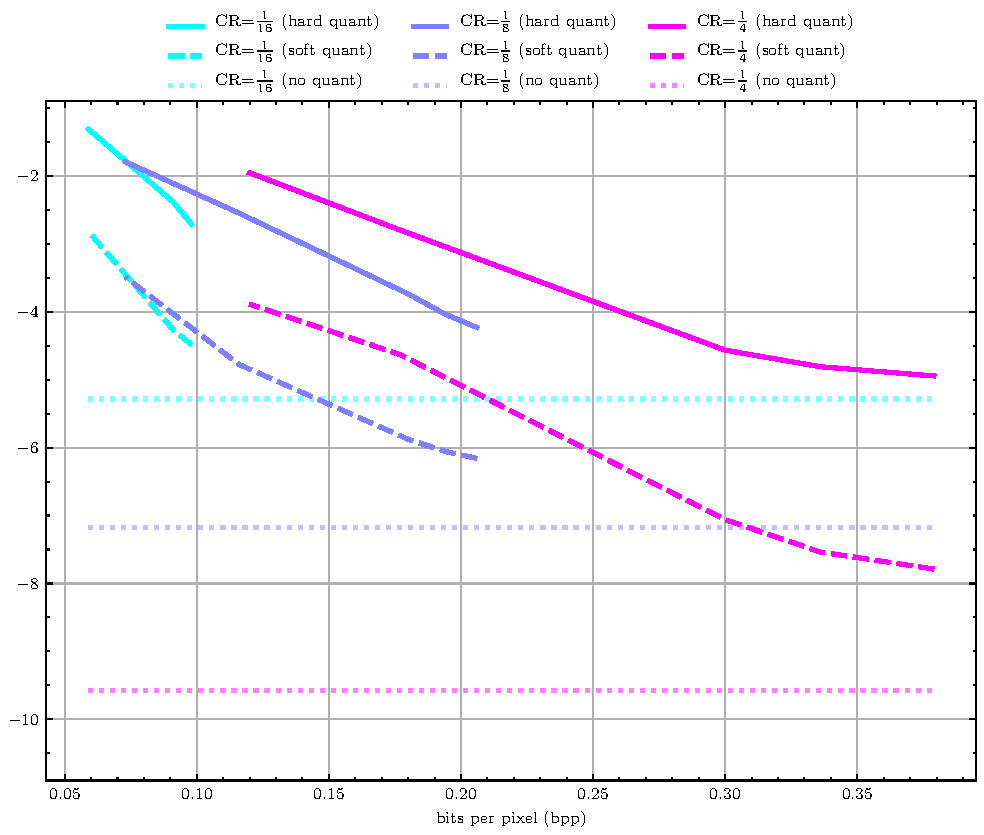
\includegraphics[width=\linewidth]{rate-distortion-all-cr-H4-K100_outdoor.pdf}
		\caption{Minmax normalization} 
		\label{fig:rate-distortion-minmax} 
	\end{subfigure}
	\begin{subfigure}[t]{.48\textwidth}
		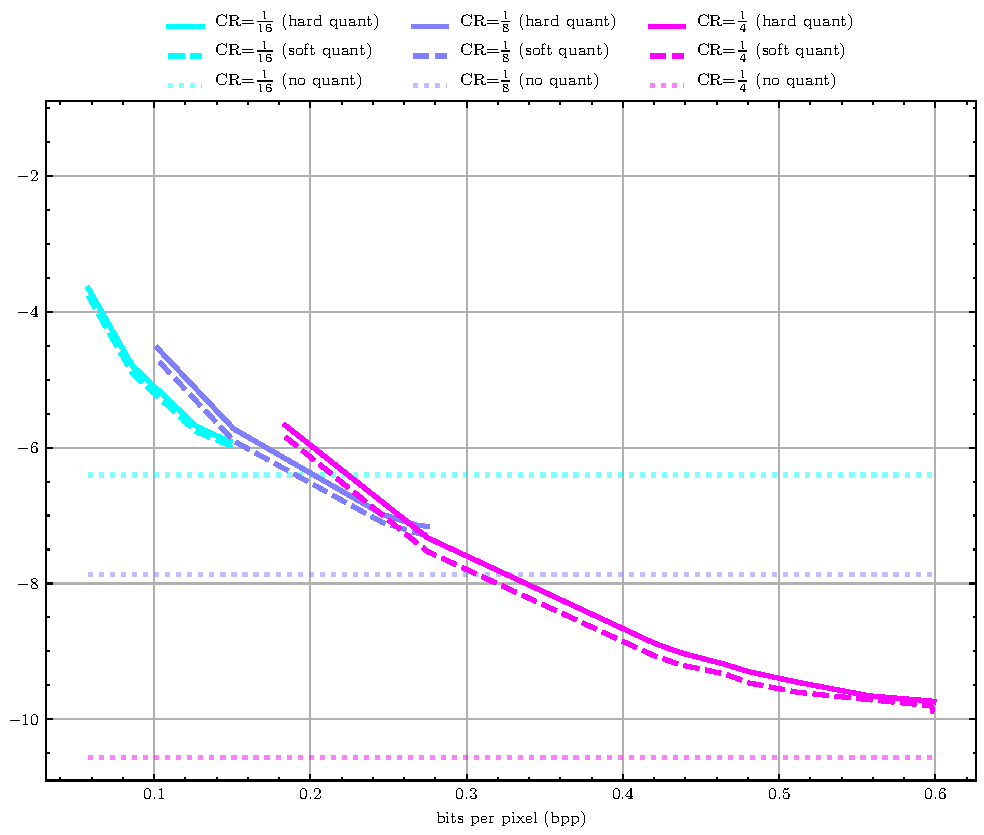
\includegraphics[width=\linewidth]{rate-distortion-all-cr-sphH4-K100_outdoor.pdf}
		\caption{Spherical normalization} 
		\label{fig:rate-distortion-sph} 
	\end{subfigure}
	\caption{Rate distortion of CsiNet-Quant trained on the outdoor network under a) minmax normalization and b) spherical normalization using: $L=1024$ centers, $d=4$. Hard, soft, and no quantization performance shown for each CR.} 
  	\label{fig:rate-distortion-softquant} 
\end{figure}

Figure~\ref{fig:rate-distortion-norms} shows the rate-distortion for both minmax and spherical normalization under hard quantization only. At comparable bit rates, the NMSE of SphNet is consistently lower than that of CsiNet-Pro, illustrating that spherical normalization enables better latent representations than minmax normalization.

\begin{figure}[htb] \centering 
  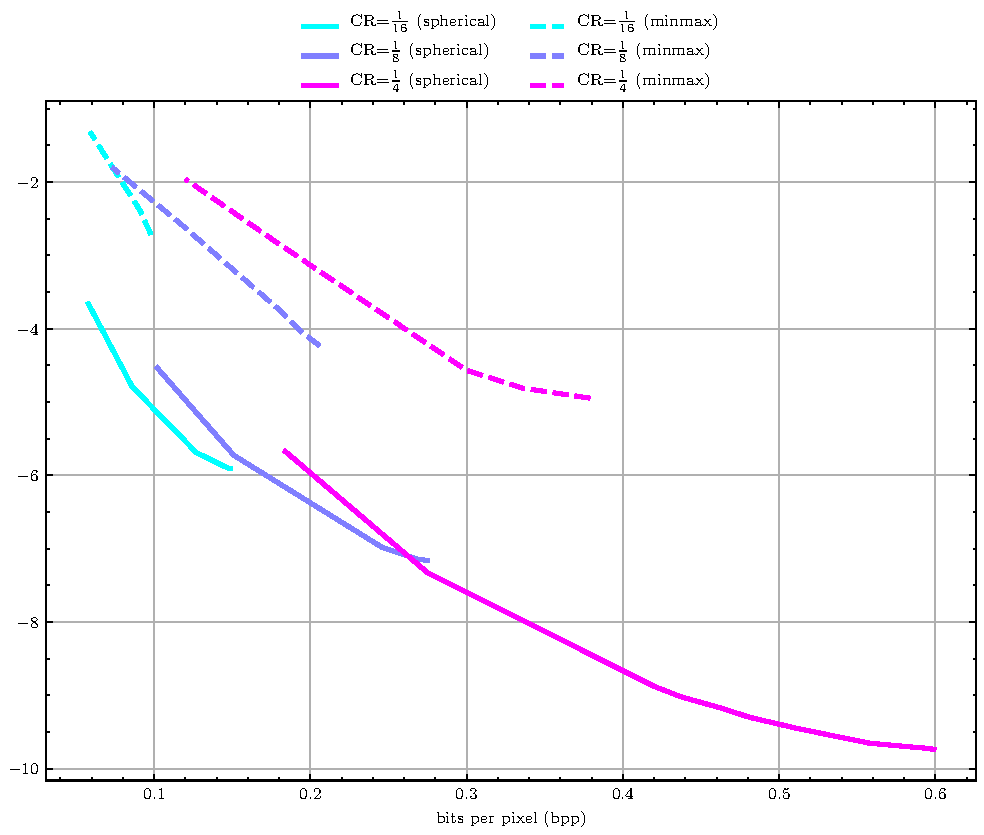
\includegraphics[width=0.55\linewidth]{rate-distortion-all-norm.pdf}
  \caption{Rate distortion of CsiNet-Quant trained on the outdoor network under hard quantization for both minmax (dotted line) and spherical (solid line) normalization.} 
  \label{fig:rate-distortion-norms} 
\end{figure}

\subsection{Results: CSI Entropy Estimation} \label{sec:results-ent-estimation}

Figure~\ref{fig:cost-ent-est} shows the estimated conditional entropy of the quantized CSI matrices ($\mathbf H^{\Delta}$) for the indoor and outdoor COST2100 channel samples. The conditional entropy is based on the following identity,
\begin{align*}
	\hat H(\mathbf H^\Delta_{t_2} | \mathbf H^\Delta_{t_1}) &= \hat H(\mathbf H^\Delta_{t_2}, \mathbf H^\Delta_{t_1}) - \hat H(\mathbf H^\Delta_{t_1})
\end{align*}
for a feedback interval $t_{\text{interval}} = t_2 - t_1$. A feedback interval of $t_{\text{interval}} = \infty$ indicates no conditioning (i.e., $\hat H(\mathbf H^\Delta_{t_2})$). Both figures show the conditional entropy for different feedback intervals, and we see that the conditional entropy for longer feedback intervals is consistently higher than that of shorter feedback intervals. 

\begin{figure}[!hbtp] \centering 
	\begin{subfigure}[t]{.48\textwidth}
		\centering
	    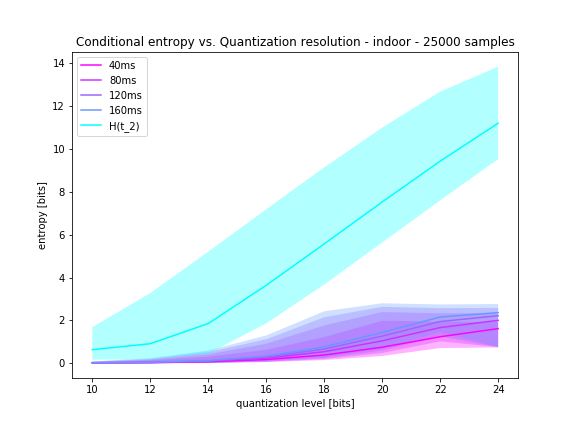
\includegraphics[width=\linewidth]{indoor_cond_entropy_25000samples_ci.png}
		\caption{Indoor}
		\label{fig:indoor_cond} 
	\end{subfigure}
  % \subfigure[Outdoor] { \label{outdoor_cond} 
	\begin{subfigure}[t]{.48\textwidth}
		\centering
		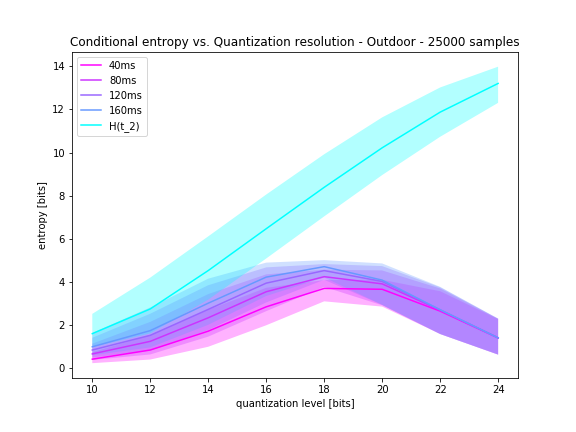
\includegraphics[width=\linewidth]{outdoor_cond_entropy_25000samples_ci.png}
		\caption{Outdoor}
		\label{fig:outdoor_cond} 
	\end{subfigure}
  % } 
  \caption{Mean entropy/conditional entropy estimates $H(\mathbf H^{\Delta})$ with 95\% c.i. for quantized i.i.d COST2100 elements vs. quantization level (bits).} 
  \label{fig:cost-ent-est} 
\end{figure}

Figure~\ref{fig:cost-diffent-est} shows the estimated conditional entropy of the quantized CSI matrices ($\mathbf H^{\Delta}$) based on the differential entropy estimates ($\hat h(\mathbf H)$). The conditional differential entropy is based on the following identity,
\begin{align*}
	\hat h(\mathbf H_{t_2} | \mathbf H_{t_1}) &= \hat h(\mathbf H_{t_2}, \mathbf H_{t_1}) - \hat h(\mathbf H_{t_1}),
\end{align*}
and the entropy of the quantized CSI matrices is obtained via Theorem 8.3.1 from Cover \cite{ref:Cover1999Elements} as defined in (\ref{eq:cover-thm}).
\begin{figure}[!hbtp] \centering 
	\begin{subfigure}[t]{.48\textwidth}
  		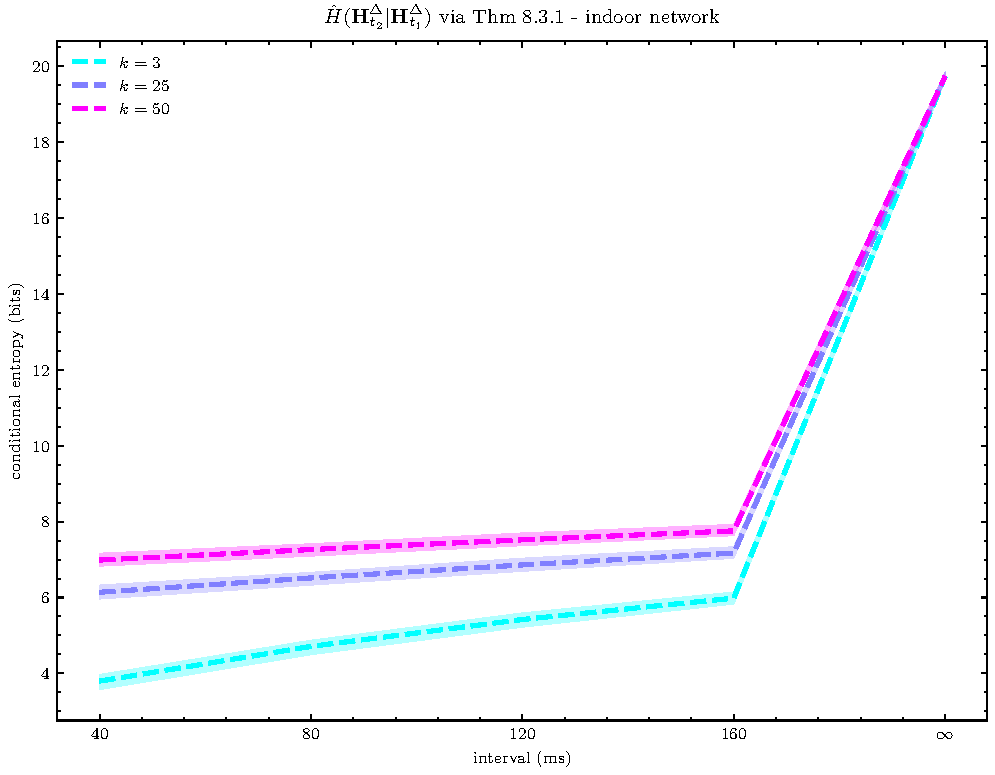
\includegraphics[width=\linewidth]{indoor_conditional_quant_joint.pdf}
		\caption{Indoor} 
		\label{fig:cost-diffent-est-indoor} 
	\end{subfigure}
	\begin{subfigure}[t]{.48\textwidth}
  		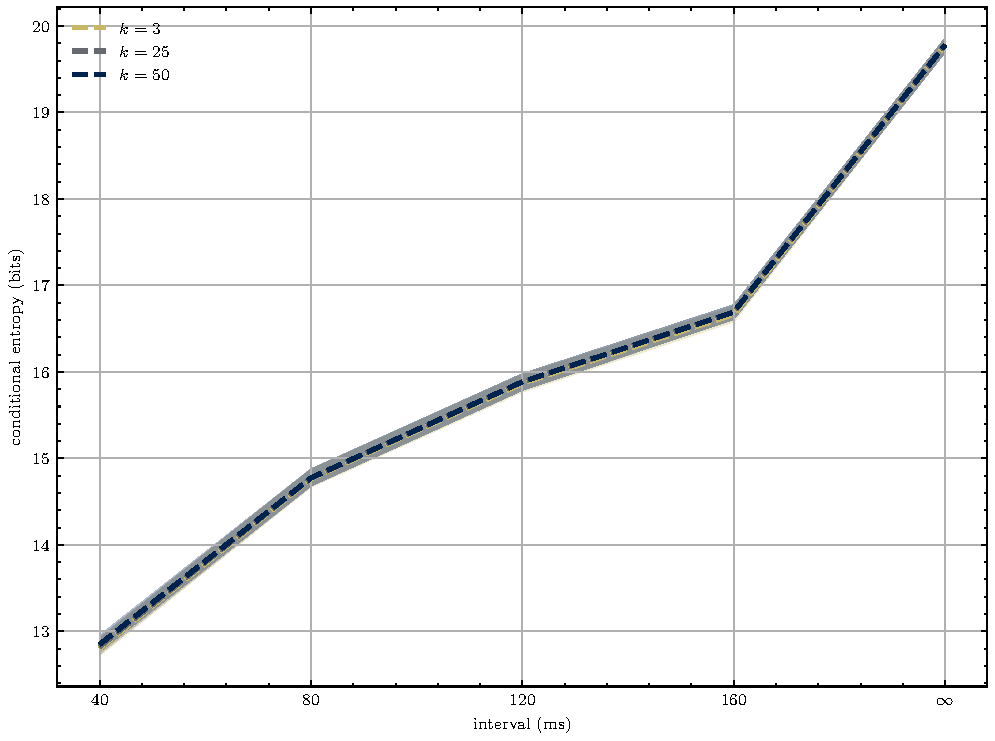
\includegraphics[width=\linewidth]{outdoor_conditional_quant_joint.pdf}
		\caption{Outdoor} 
		\label{fig:cost-diffent-est-outdoor} 
	\end{subfigure}
  \caption{Mean entropy/conditional entropy estimates $\hat H(\mathbf H^{\Delta}) = \hat h(\mathbf H) + n$ with 95\% c.i. for quantized i.i.d COST2100 elements vs. feedback interval (ms).} 
  \label{fig:cost-diffent-est} 
\end{figure}

Using $\mathbf H_\sigma^\Delta$, we can draw the rate-distortion curve for the corrupted CSI, and we can compare this curve to the achieved rate-distortion the tested networks. Figure~\ref{fig:csinet-soft-bound}) demonstrates the achieved rate-distortion under spherical normalization for CsiNet-SoftQuant. Compared with uniform quantization, SHVQ can achieve similar NMSE at lower feedback rates, but based on the bound $\hat H(\mathbf H_\sigma^\Delta)$, it is possible to achieve lower feedback bit rates at the given distortion levels. Note that the performance of CsiNet-SoftQuant was achieved with minimal hyperparameter optimization. The ultimate compression rate can likely be improved by changing the dimensionality of the codebook ($L$), the size of codewords ($m$), or training hyperparameters (see \cite{ref:Agustsson2017SoftToHard} for more details).  
% \begin{figure}[!hbtp] \centering 
% 	\begin{subfigure}[t]{.48\textwidth}
% 		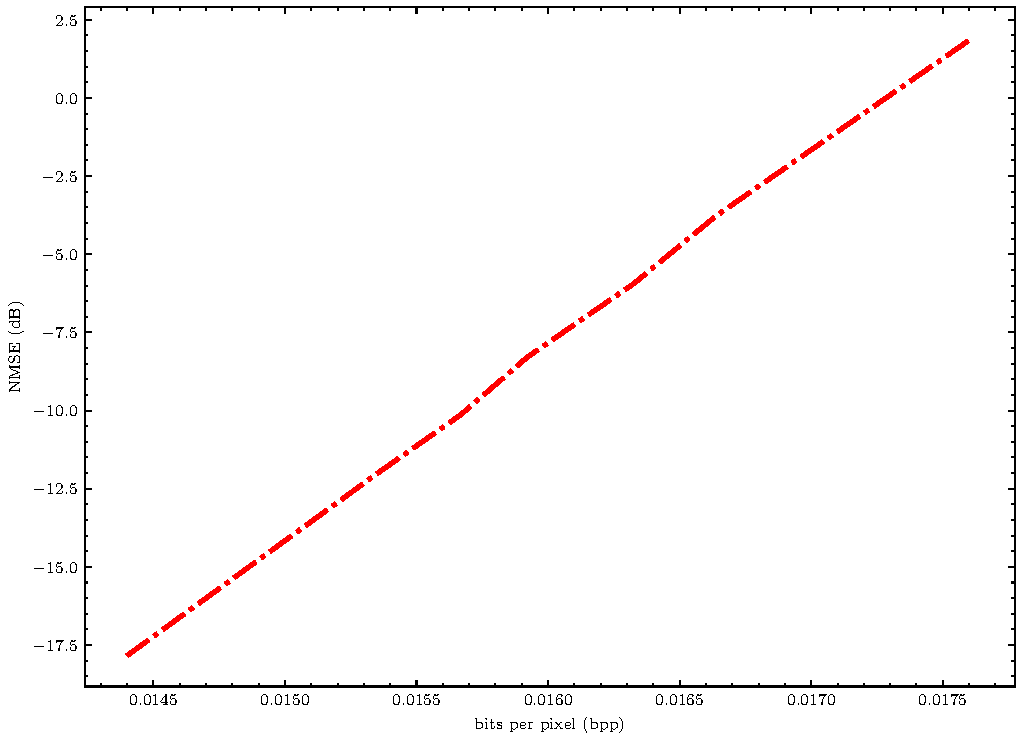
\includegraphics[width=\linewidth]{rate-distortion-gauss-bound-only-outdoor.pdf}
% 		\caption{RD bound, $\hat H(\mathbf H_\sigma^\Delta)$} 
% 		\label{fig:cost-ent-sigma} 
% 	\end{subfigure}
% 	\begin{subfigure}[t]{.48\textwidth}
% 		\centering
% 		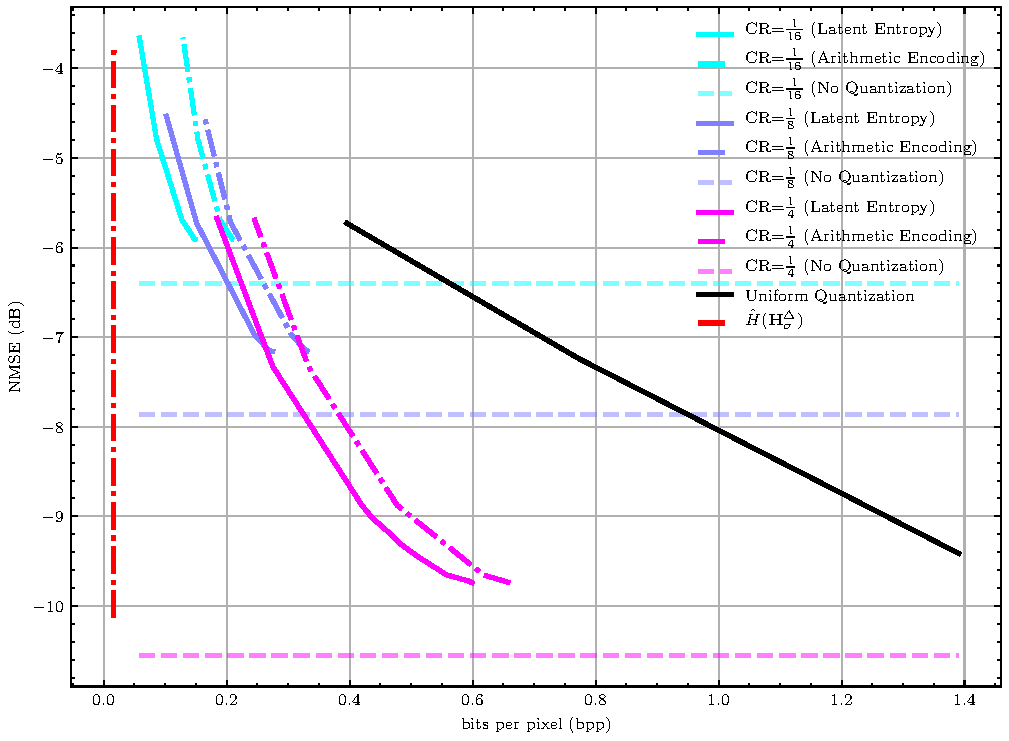
\includegraphics[width=\linewidth]{rate-distortion-with-gauss-bound-K100-outdoor.pdf}
% 		\caption{CsiNet-SoftQuant compared $\hat H(\mathbf H_\sigma^\Delta)$} 
% 		\label{fig:csinet-soft-bound} 
% 	\end{subfigure}
% \end{figure}
\begin{figure}[!hbtp] \centering 
	\centering
	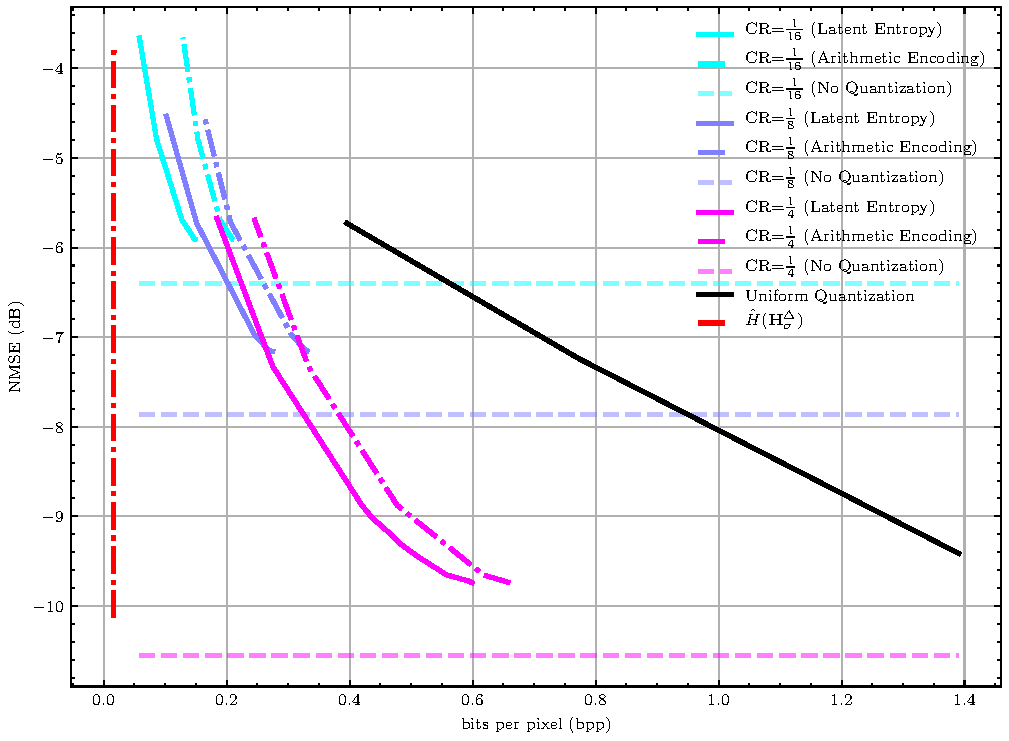
\includegraphics[width=0.55\linewidth]{rate-distortion-with-gauss-bound-K100-outdoor.pdf}
	\caption{CsiNet-SoftQuant compared to uniform quantization of latent feedback (\textbf{black}) and compared to $\hat H(\mathbf H_\sigma^\Delta)$ (\textbf{{\color{red}red}})} 
	\label{fig:csinet-soft-bound} 
\end{figure}

\section{Future Work: Rate-optimal Quantization}

Moving forward, our work in trainable CSI quantization will seek to specify networks which achieve \textbf{rate-optimal quantization}. A rate-optimal network will achieve feedback entropy approaching the entropy of the underlying CSI matrices. In addition to hyperparameter optimization (as discussed in Section~\ref{sec:results-ent-estimation}) and different quantization frameworks (e.g., $\text{MCR}^2$ \cite{ref:Yu2020MCR2}), we plan to investigate the following two avenues to achieve rate-optimal CSI compression.

\subsection{ROI CSI Compression}

\begin{figure}[htb] \centering 
	\begin{subfigure}[t]{.48\textwidth}
		\input{../images/batch0_csi_roi_lo.pdf_tex}
		\caption{Low threshold} 
		\label{fig:roi-lo} 
	\end{subfigure}
	\begin{subfigure}[t]{.48\textwidth}
		\input{../images/batch0_csi_roi_hi.pdf_tex}
		\caption{High threshold} 
		\label{fig:roi-hi} 
	\end{subfigure}
	\caption{Hypothetical bounding boxes based on threshold, $\tau$, where $\tau_{\text{lo}} < \tau_{\text{hi}}$. The set of ROI pixels constitute $\mathbf S_{\text{ROI}}$.} 
  	\label{fig:roi-thresh} 
\end{figure}

Region of interest (ROI) based compression emphasizes the encoding and decoding of designated sections of a given signal. By labeling ground truth ROIs, the network can be penalized based on the rate of these ROIs. For example, in the case of a CSI matrix $\mathbf H$ with a set of ROI elements, $\mathbf S_{\text{ROI}}$, the MSE of the ROI can be written as
\begin{align*}
	L_{\text{MSE,ROI}} &= \frac{1}{N_{\text{ROI}}} \sum_{i\in\mathbf S_{\text{ROI}}}\Arrowvert \mathbf H_i - g(f(\mathbf H_i, \theta_e), \theta_d) \Arrowvert^2.
	% L_{\text{Rate,ROI}} &= \frac{1}{N_{\text{ROI}}} \sum_{i\in\mathbf S_{\text{ROI}}} \log_2(\mathbf H_i).
\end{align*}
Deep learning-based ROI compression has demonstrated success in image compression tasks, demonstrating lower distortion at lower rates compared to non-ROI image codecs \cite{ref:Cai2020EndToEndOptimizedROIImageCompression}. Given the sparsity of CSI in the angular-delay domain, ground truth ROI masks can be chosen to capture the dominant non-zero elements. In this line of investigation, a variety of metrics will be used to establish ground truth masks, such bounding boxes based on magnitude thresholding (e.g., Figure~\ref{fig:roi-thresh}). 

\subsection{Differential Encoding with Trainable Feedback Quantization}

As highlighted by our entropy estimation experiments (Figures~\ref{fig:cost-ent-est} and~\ref{fig:cost-diffent-est}), the conditional entropy $\hat H(\mathbf H_{t_2}|\mathbf H_{t_1})$ is appreciably lower than the entropy $\hat H(\mathbf H_{t_2})$. The resulting entropy reduction implies a corresponding reduction in feedback rate for compressed CSI. Our future work will investigate the compatibility of differential encoding (see Section~\ref{chap:markovnet}) with trainable feedback quantization. We anticipate that the achieved bit rates for quantized differential encoders should be substantially lower than non-temporal encoders.
